% --------------------------------------------------------------
% This is all preamble stuff that you don't have to worry about.
% Head down to where it says "Start here"
% --------------------------------------------------------------

\documentclass[12pt]{article}

\usepackage[margin=1in]{geometry}
\usepackage{times}
\usepackage{amsmath,amsthm,amssymb}
\usepackage{caption}
\usepackage{graphicx,subfigure}
\usepackage{listings}
\usepackage{url}

\newcommand{\N}{\mathbb{N}}
\newcommand{\Gauss}{\mathcal{N}}
\newcommand{\Z}{\mathbb{Z}}
\newcommand{\E}{\mathbb{E}}
\newcommand{\R}{\mathbb{R}}
\newcommand{\p}{{\bf p}}
\newcommand{\1}{\mathbf{1}}

% \linespread{0}

\newenvironment{theorem}[2][Theorem]{\begin{trivlist}
\item[\hskip \labelsep {\bfseries #1}\hskip \labelsep {\bfseries #2.}]}{\end{trivlist}}
\newenvironment{lemma}[2][Lemma]{\begin{trivlist}
\item[\hskip \labelsep {\bfseries #1}\hskip \labelsep {\bfseries #2.}]}{\end{trivlist}}
\newenvironment{claim}[2][Claim]{\begin{trivlist}
\item[\hskip \labelsep {\bfseries #1}\hskip \labelsep {\bfseries #2.}]}{\end{trivlist}}
\newenvironment{exercise}[2][Exercise]{\begin{trivlist}
\item[\hskip \labelsep {\bfseries #1}\hskip \labelsep {\bfseries #2.}]}{\end{trivlist}}
\newenvironment{problem}[2][Problem]{\begin{trivlist}
\item[\hskip \labelsep {\bfseries #1}\hskip \labelsep {\bfseries #2.}]}{\end{trivlist}}
\newenvironment{question}[2][Question]{\begin{trivlist}
\item[\hskip \labelsep {\bfseries #1}\hskip \labelsep {\bfseries #2.}]}{\end{trivlist}}
\newenvironment{corollary}[2][Corollary]{\begin{trivlist}
\item[\hskip \labelsep {\bfseries #1}\hskip \labelsep {\bfseries #2.}]}{\end{trivlist}}

\begin{document}
{\raggedright

% --------------------------------------------------------------
%                         Start here
% --------------------------------------------------------------

\title{ECE 544NA HW3}%replace X with the appropriate number
\author{Jiaqi Mu~jiaqimu2 \\
% collaborating with Hongyu Gong~hgong6 \\
[8pt]%replace with your name
Department of Electrical and Computer Engineering} %if necessary, replace with your course title

\maketitle

\section{Pencil-and-Paper\label{sec:1}}
In this part of the assignment, you will derive the update equations for Gaussian Mixture Models using the EM algorithm. You are given a dataset, $D=\{x_1, ..., x_n\}$. You have reason to believe that $p_{X|\Theta}(x_i | \theta)$ can be modeled as,
\begin{align*}
  p_{X|\Theta}(x_i | \theta) = \sum_{h=1}^m w_h p_{V|H, \Theta}(x, h, \theta),
\end{align*}
where $p_{V|H,\Theta}(x, h, \theta)$ has the form of a Gaussian distribution, and $\sum_{k=1}^m w_k=1$. We also define the posterior probability with the following notation.
\begin{align*}
  \gamma_i(k) = \frac{w_k \mathcal{N}(x_i; \mu_k, \Sigma_k)}{\sum_l w_l \mathcal{N}(x_i; \mu_l, \Sigma_l)}
\end{align*}

\begin{itemize}
  \item Read {\em A gentle tutorial of the EM algorithm and its application to parameter estimation for Gaussian mixture and hidden Markov models}, to review the EM algorithm and GMM.
  \item Write out the E-Step equations, following the notation above.
  \begin{proof}
    The expectation step is to find $Q(\theta | \theta^{(t)})$ given $\theta^{(t)}$, from where we know the hidden random variable is $H$ and the observed random variable is $X$. Thus given the posterior probability distribution $\gamma_i$ on $H_i$, we have,
    \begin{align*}
      Q(\theta | \theta^{(t)}) &= \E_{H|X, \theta^{(t)}} \log L(\theta; x, H) \\
      &= \sum_{h=1}^m \sum_{i=1}^n P(H_i = h | X_i = x_i;\theta^{(t)}) \log L(\theta_h; x_i, h) \\
      &= \sum_{h=1}^m \sum_{i=1}^n \log (w_h \mathcal{N}(x_i; \mu_h, \Sigma_h)) \gamma_i(h) \\
      &= \sum_{h=1}^m \gamma_i(h) \left(\log w_h - \frac{1}{2}\log |\Sigma_h| - \frac{1}{2}(x_i - \mu_h)^{\rm T} \Sigma_h^{-1} (x_i - \mu_h) - \frac{d}{2} \log (2\pi) \right),
    \end{align*}
    where $d$ is the dimension for $X$, and $\gamma$ is a posterior probability distribution, defined as,
    \begin{align}
      \gamma_i(k) = \frac{w_k^{(t)} \mathcal{N}(x_i; \mu_k^{(t)}, \Sigma_k^{(t)})}{\sum_l w_l^{(t)} \mathcal{N}(x_i; \mu_l^{(t)}, \Sigma_l^{(t)})} \label{eq:estep}
    \end{align}
    In this specific problem, only \eqref{eq:estep} is required for computational purpose.
  \end{proof}
  \item Write out the M-Step equations, following the notation above.
  \begin{proof}
    The maximization step is to get $\theta$ that maximize $Q(\theta|\theta^{t})$, in our case $\theta = \left(w_h, \mu_h, \Sigma_h\right)_{h=1}^m$. The updating parameters are given as follow,
    \begin{align}
      w_h^{(t+1)} &= \frac{1}{n} \sum_{i=1}^n \gamma_i(h) , \label{eq:weight}\\
      \mu_h^{(t+1)}&= \frac{\sum_{i=1}^n x_i \gamma_i(h)}{\sum_{i=1}^n \gamma_i(h)} , \label{eq:mean}\\
      \Sigma_h^{(t+1)} &= \frac{\sum_{i=1}^n \gamma_i(h) \left(x_i - \mu_h^{(t+1)}\right)\left(x_i - \mu_h^{(t+1)}\right)^{\rm T}}{\sum_{i=1}^n \gamma_i(h)}. \label{eq:variance}
    \end{align}
  \end{proof}
\end{itemize}

\section{Code-From-Scratch}
In this portion of the assignment, you'll be clustering an image based on colors. Humans naturally group similar colors together; for example, we might describe a particular outfit as ``a maroon sweater with navy blue shorts,'' ignoring the many subtle variations of color tone present in the sweater.

Given an image, we denote $\vec{x}[\vec{n}] = [r_{\vec{n}}, g_{\vec{n}}, b_{\vec{n}}]^{\rm T}$ as the RGB color vector at pixel $\vec{n} = [n_1, n_2]$ of an image. We treat each pixel as independent examples, meaning we have a training set of $\{\vec{x}_i\}$, where $i$ is the linear index mapped from $\vec{n}$.

Train a Gaussian Mixture model on $\{\vec{x}_i\}$, using the EM update equations derived in Pencil-and-Paper portion of the assignment. Here, we assume $m=3$, , this model is a mixture of 3 Gaussian distributions. Randomly initialize the $\mu$ and $\sigma$ for each of the Gaussian distribution.

With a trained GMM, you will have the following values $w_1, w_2, w_3, \vec{\mu}_1, \vec{\mu}_2, \vec{\mu}_3, \Sigma_1, \Sigma_2, \Sigma_3$ include these in your report.

Lastly, assign a cluster label for each of the pixels in the image. This can be done by computing likelihood that the example $x_{\vec{n}}$ comes from each of the Gaussian distribution in the mixture, and picking the maximum. Denote the cluster label as $l^*$. With the cluster label, now compute an image, where the pixel $x_{\vec{n}}$ is replaced with the corresponding cluster mean $\mu_{l^*}$.

Repeat with different number of clusters, $m=5$ and $m=10$.

\subsection{Modules}
Note: For this assigment you are required to have the following modules
\begin{itemize}
  \item Create a function {\tt gammaprob} that accepts the parameters of a Gaussian mixture model (GMM), in any format that you find convenient (you'll have to use this format for the rest of this problem set), and the data samples as input, and outputs the posterior probability vectors
  \item A function {\tt estep} that computes the E-step for training a Gaussian mixture model.
  \item A function {\tt mstep} that computes the M-step for training a Gaussian mixture model.
\end{itemize}

\subsection{Methods}
\begin{itemize}
  \item Describe the functions you wrote, and the overall structure of your code.
  \begin{proof}
    In my implementation, I create two functions to read and save data, create one class for GMM:
    \begin{itemize}
      \item {\tt data.py} contains two functions:
      \begin{itemize}
        \item {\tt readData}: to read rgb values from a image and convert them into an array
        \item {\tt saveData}: to save rgb arrays to an output image
      \end{itemize}
      \item {\tt gmm.py} contains a GMM class:
      \begin{itemize}
        \item {\tt \_\_init\_\_}: to initialize parameters, i.e., the number of clusters, a random seed, and the iterations
        \item {\tt gammaprob}: to compute the posterior probabilities
        \item {\tt fit}: to fit the model into data. This function contains two sub-functions:
        \begin{itemize}
          \item {\tt estep}: is the expectation step by calling {\tt gammaprob} to compute the posterior probabilities
          \item {\tt mstep}: is to update the cluster centers, covariance matrices, and weights for each cluster.
        \end{itemize}
        \item {\tt predict}: to predict the cluster index for a new instance
        \item {\tt clusters}: to return the cluster centers
        \item {\tt covariances}: to return the covariance matrices.
      \end{itemize}
    \end{itemize}
  \end{proof}
  \item How many trainable parameters are in the GMM model?
  \begin{proof}
    The trainable parameters are $\vec{\mu}$'s, $\Sigma$'s, and $w$'s, which in total is,
    \begin{align*}
      N \times ( D + D^2 + 1),
    \end{align*}
    where $N$ is the number of cluster, and $D$ is the dimension for training data.
  \end{proof}
\end{itemize}

\subsection{Results}
\begin{itemize}
  \item Report the following  $w_1, w_2, w_3, \vec{\mu}_1, \vec{\mu}_2, \vec{\mu}_3, \Sigma_1, \Sigma_2, \Sigma_3$ for $m=3$.
  \begin{proof}
    Using the default image with $m=3$, we have the output image as reported in Figure~\ref{fig:part3-1}(a), and the parameters below:
      \begin{align*}
w_{1} &= 0.33 \\
\vec{\mu}_{1} &= \begin{bmatrix} 193.91 &  151.68 &  105.95 &  \end{bmatrix} \\
\Sigma_{1} &= \begin{bmatrix} 1324.43 &  1383.86 &  1491.69 &  \\1383.86 &  1618.27 &  1829.14 &  \\1491.69 &  1829.14 &  2284.88 &  \end{bmatrix} \\
w_{2} &= 0.48 \\
\vec{\mu}_{2} &= \begin{bmatrix} 88.28 &  99.96 &  0.31 &  \end{bmatrix} \\
\Sigma_{2} &= \begin{bmatrix} 2428.88 &  2569.89 &  -19.77 &  \\2569.89 &  2916.18 &  -21.85 &  \\-19.77 &  -21.85 &  0.37 &  \end{bmatrix} \\
w_{3} &= 0.19 \\
\vec{\mu}_{3} &= \begin{bmatrix} 94.23 &  87.72 &  22.08 &  \end{bmatrix} \\
\Sigma_{3} &= \begin{bmatrix} 1763.93 &  1648.48 &  153.49 &  \\1648.48 &  2021.27 &  10.59 &  \\153.49 &  10.59 &  301.75 &  \end{bmatrix} \\
\end{align*}


    \begin{figure}[htbp]
    \centering
    \subfigure[original]
    {
    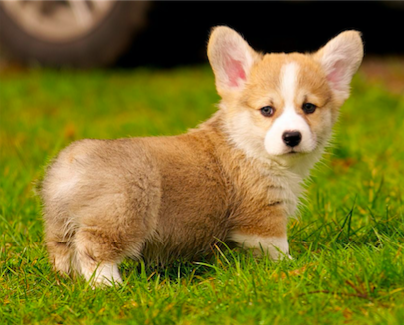
\includegraphics[width=0.22\textwidth]{../data/hw3.png}
    }
    \subfigure[$m=3$]
    {
    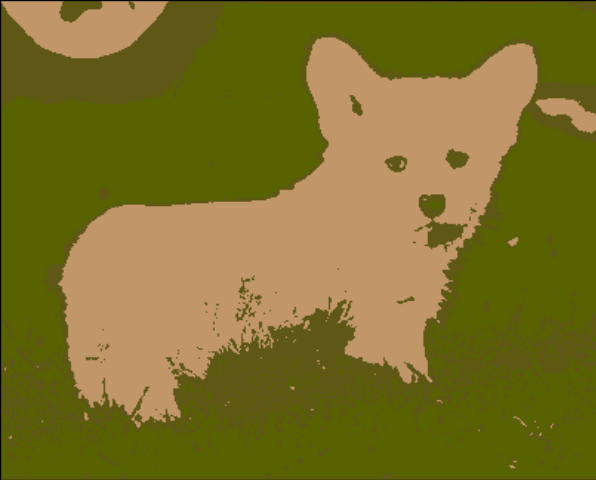
\includegraphics[width=0.22\textwidth]{../figures/hw3-part2-3.png}
    }
    \subfigure[$m=5$]
    {
    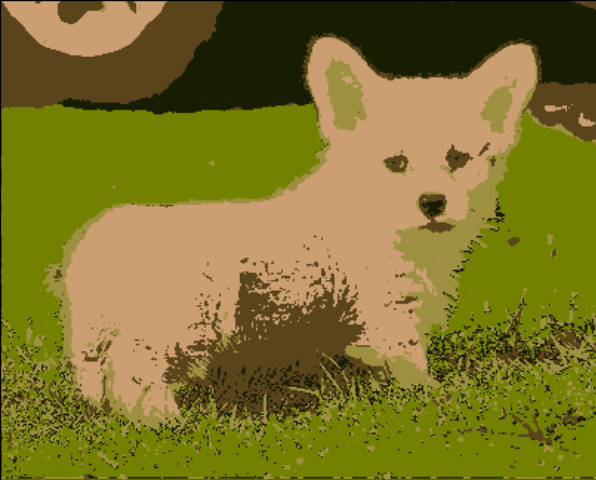
\includegraphics[width=0.22\textwidth]{../figures/hw3-part2-5.png}
    }
    \subfigure[$m=10$]
    {
    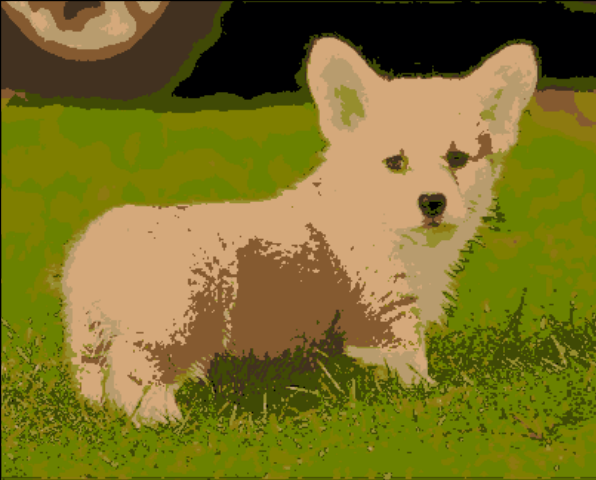
\includegraphics[width=0.22\textwidth]{../figures/hw3-part2-10.png}
    }
    \caption{Output for default image with $m=3,5,10$.\label{fig:part2-1}}
    \end{figure}

  \end{proof}
  \item Include the image after clustering for $m=3$, $m=5$, and $m=10$.
  \begin{proof}
    The image for $m=3$, $m=5$ and $m=10$ are listed in Figure~\ref{fig:part2-1}.
  \end{proof}
  \item Repeat 1. and 2. on another image of your choice.

  \begin{proof}
    We repeat the experiment on the image in Figure~\ref{fig:part2-2}(a). The output image for $m=3$, $m=5$ and $m=10$ are also reported in Figure~\ref{fig:part2-2}(b-d). The parameters for $m=3$ are as follow:
    \begin{align*}
    w_{1} &= 0.21 \\
\vec{\mu}_{1} &= \begin{bmatrix} 193.30 &  183.74 &  171.47 &  \end{bmatrix} \\
\Sigma_{1} &= \begin{bmatrix} 1472.59 &  1514.62 &  1508.15 &  \\1514.62 &  1651.25 &  1742.23 &  \\1508.15 &  1742.23 &  1970.06 &  \end{bmatrix} \\
w_{2} &= 0.56 \\
\vec{\mu}_{2} &= \begin{bmatrix} 56.54 &  72.74 &  91.42 &  \end{bmatrix} \\
\Sigma_{2} &= \begin{bmatrix} 550.06 &  716.62 &  812.44 &  \\716.62 &  1039.04 &  1232.28 &  \\812.44 &  1232.28 &  1495.36 &  \end{bmatrix} \\
w_{3} &= 0.23 \\
\vec{\mu}_{3} &= \begin{bmatrix} 127.39 &  87.37 &  45.33 &  \end{bmatrix} \\
\Sigma_{3} &= \begin{bmatrix} 2165.75 &  1954.19 &  1298.90 &  \\1954.19 &  1954.07 &  1386.44 &  \\1298.90 &  1386.44 &  1174.10 &  \end{bmatrix} \\
\end{align*}


    \begin{figure}[htbp]
    \centering
    \subfigure[original]
    {
    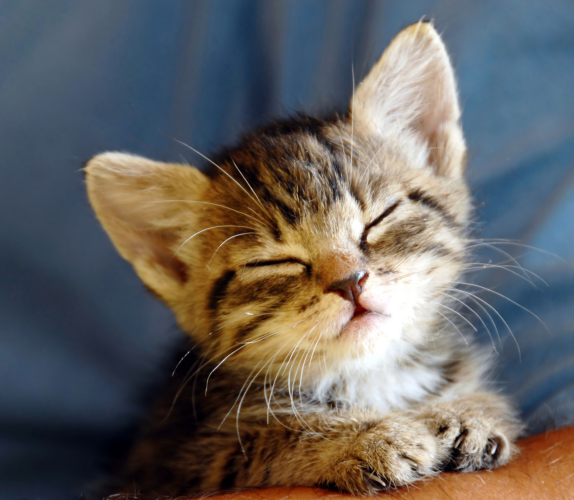
\includegraphics[width=0.22\textwidth]{../data/cat.png}
    }
    {
    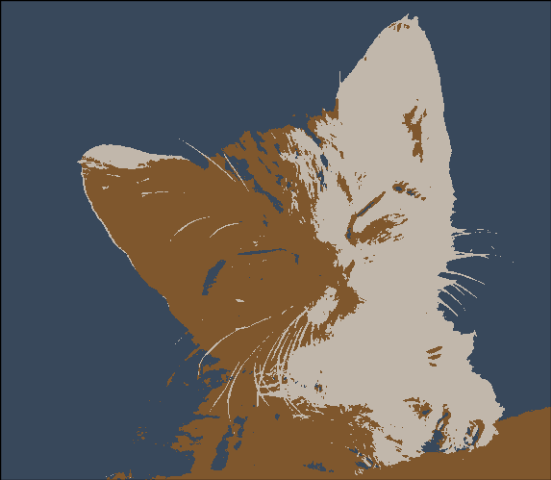
\includegraphics[width=0.22\textwidth]{../figures/cat-part2-3.png}
    }
    \subfigure[$m=5$]
    {
    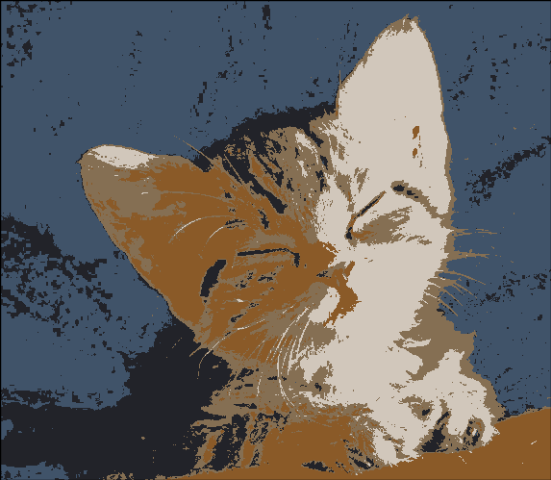
\includegraphics[width=0.22\textwidth]{../figures/cat-part2-5.png}
    }
    \subfigure[$m=10$]
    {
    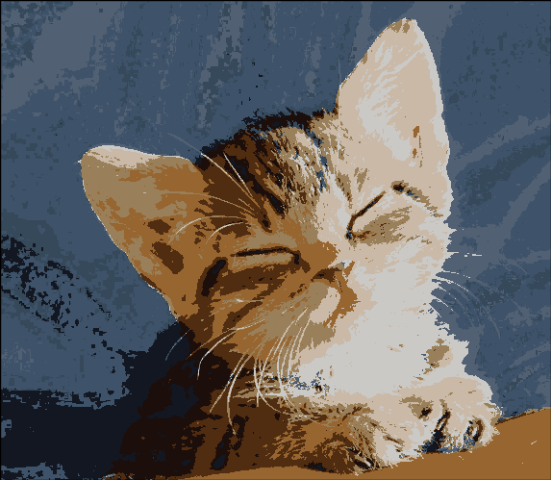
\includegraphics[width=0.22\textwidth]{../figures/cat-part2-10.png}
    }
    \caption{Output for custom-chose image with $m=3,5,10$.\label{fig:part2-2}}
    \end{figure}
  \end{proof}
\end{itemize}

\section{TensorFlow}
In this section, you will use a higher-level API from the TensorFlow GMM\footnote{\url{https://github.com/tensorflow/tensorflow/blob/32bd3d024f33e920a67a1081bc0ae0048350fdee/tensorflow/contrib/factorization/python/ops/gmm.py}}, to repeat the code-from-scratch task described above.

\subsection{Methods}
\begin{itemize}
  \item Describe the functions you wrote, and the overall structure of your code.
  \begin{proof}
    In this part, we reuse {\tt readData} and {\tt saveData} from part 2 to load image and print image. For each image and each parameter, we do the following steps:
    \begin{itemize}
      \item Load image using {\tt readData}.
      \item Initialize a GMM class by calling {gmm = \tt GMM()}.
      \item Train the parameters within this class by fitting the data using {\tt gmm.fit(data)}.
      \item Predict the cluster index for each sample by calling {\tt gmm.predict(sample)}.
      \item Construct an output image using the cluster centers and cluster indices.
      \item Output the image using {\tt saveData}
    \end{itemize}
  \end{proof}
\end{itemize}

\subsection{Results}
\begin{itemize}
  \item Report the following  $w_1, w_2, w_3, \vec{\mu}_1, \vec{\mu}_2, \vec{\mu}_3, \Sigma_1, \Sigma_2, \Sigma_3$ for $m=3$.
  \begin{proof}
    Using the default image with $m=3$, we have the output image as reported in Figure~\ref{fig:part3-1}(a), and the parameters below:
      \begin{align*}
w_{1} & = 0.29 \\
\vec{\mu}_{1} &= \begin{bmatrix} 195.57 &  152.18 &  106.99 &  \end{bmatrix} \\
\Sigma_{1} &= \begin{bmatrix} 1483.73 &  1611.09 &  1665.41 &  \\1611.09 &  1882.66 &  2005.42 &  \\1665.41 &  2005.42 &  2342.50 &  \end{bmatrix} \\
w_{2} & = 0.41 \\
\vec{\mu}_{2} &= \begin{bmatrix} 110.51 &  125.94 &  0.00 &  \end{bmatrix} \\
\Sigma_{2} &= \begin{bmatrix} 446.58 &  286.39 &  0.00 &  \\286.38 &  323.65 &  0.00 &  \\0.00 &  0.00 &  0.00 &  \end{bmatrix} \\
w_{3} & = 0.30 \\
\vec{\mu}_{3} &= \begin{bmatrix} 50.14 &  43.76 &  15.39 &  \end{bmatrix} \\
\Sigma_{3} &= \begin{bmatrix} 3412.27 &  2922.48 &  788.28 &  \\2922.48 &  2667.03 &  598.36 &  \\788.28 &  598.36 &  443.04 &  \end{bmatrix} \\
\end{align*}

    \begin{figure}[htbp]
    \centering
    \subfigure[original]
    {
    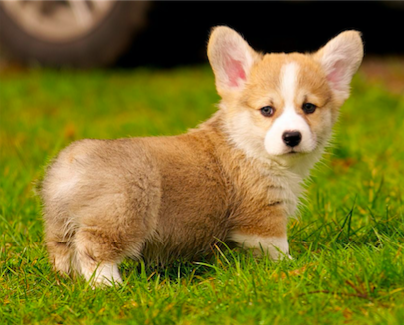
\includegraphics[width=0.22\textwidth]{../data/hw3.png}
    }
    \subfigure[$m=3$]
    {
    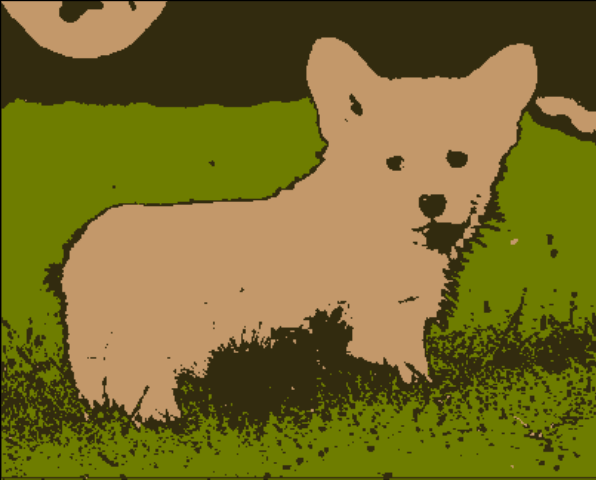
\includegraphics[width=0.22\textwidth]{../figures/hw3-part3-3.png}
    }
    \subfigure[$m=5$]
    {
    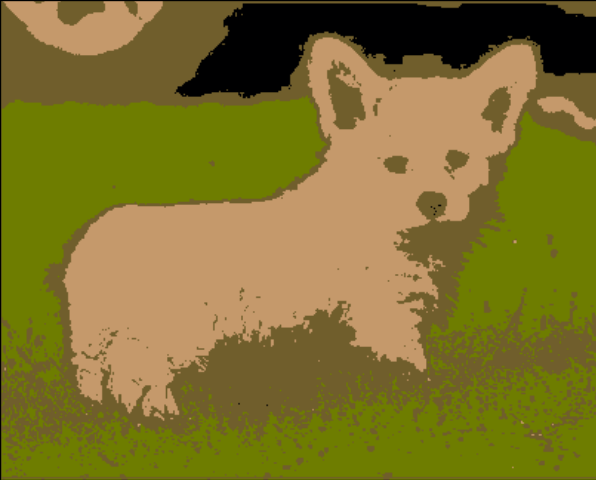
\includegraphics[width=0.22\textwidth]{../figures/hw3-part3-5.png}
    }
    \subfigure[$m=10$]
    {
    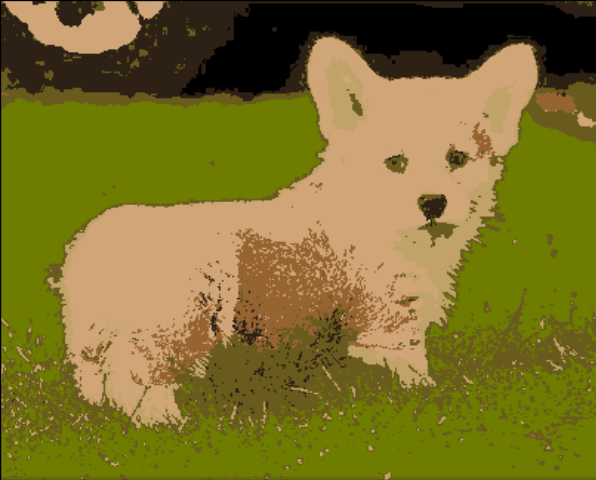
\includegraphics[width=0.22\textwidth]{../figures/hw3-part3-10.png}
    }
    \caption{Output for default image with $m=3,5,10$.\label{fig:part3-1}}
    \end{figure}

  \end{proof}
  \item Include the image after clustering for $m=3$, $m=5$, and $m=10$.
  \begin{proof}
    The image for $m=3$, $m=5$ and $m=10$ are listed in Figure~\ref{fig:part3-1}.
  \end{proof}
  \item Repeat 1. and 2. on another image of your choice.
  \begin{proof}
    We repeat the experiment on the image in Figure~\ref{fig:part3-2}(a). The output image for $m=3$, $m=5$ and $m=10$ are also reported in Figure~\ref{fig:part3-2}(b-d). The parameters for $m=3$ are as follow:
    \begin{align*}
w_{1} & = 0.15 \\
\vec{\mu}_{1} &= \begin{bmatrix} 192.29 &  166.79 &  144.04 &  \end{bmatrix} \\
\Sigma_{1} &= \begin{bmatrix} 1527.09 &  2215.34 &  2572.88 &  \\2215.34 &  3502.16 &  4166.52 &  \\2572.88 &  4166.52 &  5073.26 &  \end{bmatrix} \\
w_{2} & = 0.24 \\
\vec{\mu}_{2} &= \begin{bmatrix} 98.41 &  69.64 &  36.52 &  \end{bmatrix} \\
\Sigma_{2} &= \begin{bmatrix} 3750.18 &  3114.04 &  1584.00 &  \\3114.04 &  2681.40 &  1484.26 &  \\1584.00 &  1484.26 &  1036.27 &  \end{bmatrix} \\
w_{3} & = 0.61 \\
\vec{\mu}_{3} &= \begin{bmatrix} 73.48 &  88.79 &  106.65 &  \end{bmatrix} \\
\Sigma_{3} &= \begin{bmatrix} 1463.77 &  1330.35 &  1126.62 &  \\1330.35 &  1298.77 &  1173.27 &  \\1126.62 &  1173.27 &  1123.96 &  \end{bmatrix} \\
\end{align*}
    \begin{figure}[htbp]
    \centering
    \subfigure[original]
    {
    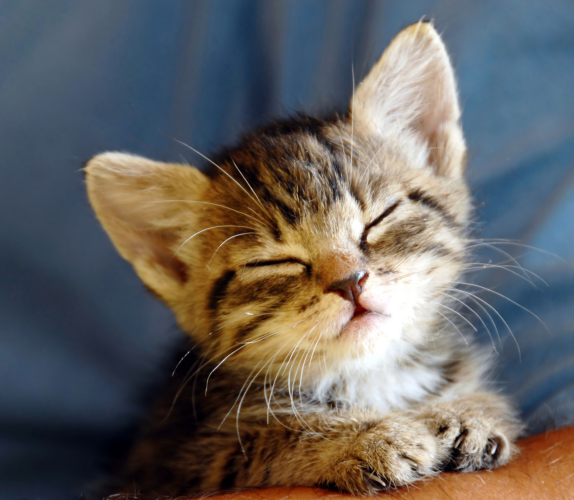
\includegraphics[width=0.22\textwidth]{../data/cat.png}
    }
    {
    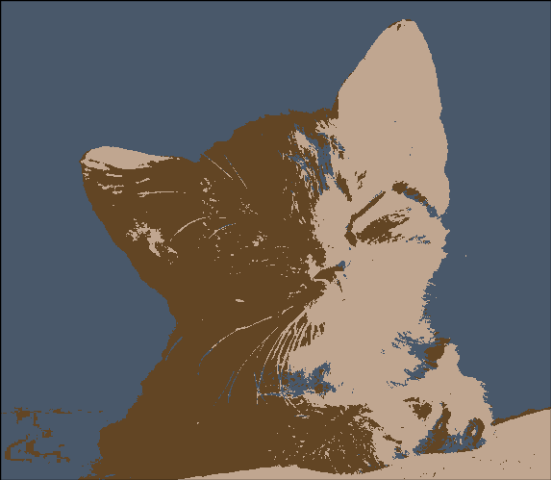
\includegraphics[width=0.22\textwidth]{../figures/cat-part3-3.png}
    }
    \subfigure[$m=5$]
    {
    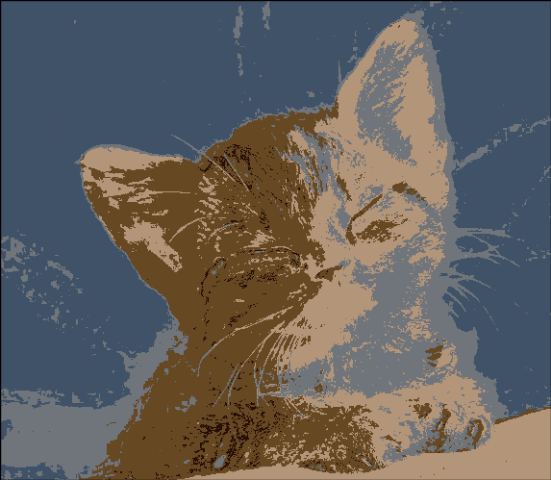
\includegraphics[width=0.22\textwidth]{../figures/cat-part3-5.png}
    }
    \subfigure[$m=10$]
    {
    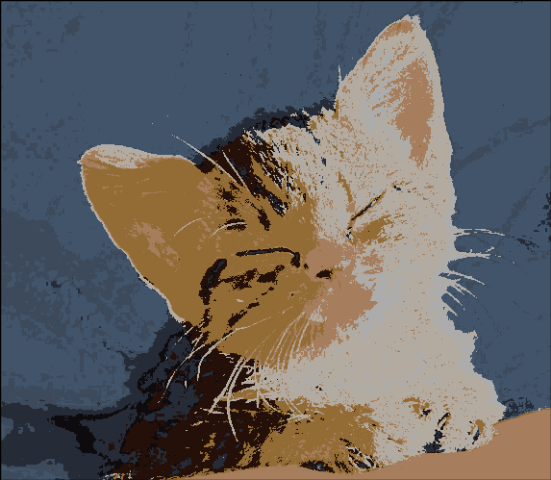
\includegraphics[width=0.22\textwidth]{../figures/cat-part3-10.png}
    }
    \caption{Output for custom-chose image with $m=3,5,10$.\label{fig:part3-2}}
    \end{figure}
  \end{proof}
\end{itemize}

\par}
\end{document}
